% Options for packages loaded elsewhere
\PassOptionsToPackage{unicode}{hyperref}
\PassOptionsToPackage{hyphens}{url}
\documentclass[
  english,
  russian,
  12pt,
  a4paper,
]{scrreprt}
\usepackage{xcolor}
\usepackage{amsmath,amssymb}
\setcounter{secnumdepth}{-\maxdimen} % remove section numbering
\usepackage{iftex}
\ifPDFTeX
  \usepackage[T1]{fontenc}
  \usepackage[utf8]{inputenc}
  \usepackage{textcomp} % provide euro and other symbols
\else % if luatex or xetex
  \usepackage{unicode-math} % this also loads fontspec
  \defaultfontfeatures{Scale=MatchLowercase}
  \defaultfontfeatures[\rmfamily]{Ligatures=TeX,Scale=1}
\fi
\usepackage{lmodern}
\ifPDFTeX\else
  % xetex/luatex font selection
  \setmainfont[Ligatures=Common,Ligatures=TeX,Scale=0.94]{IBM Plex
Serif}
  \setsansfont[Ligatures=Common,Ligatures=TeX,Scale=MatchLowercase,Scale=0.94]{IBM
Plex Sans}
  \setmonofont[Scale=MatchLowercase,Scale=0.94,FakeStretch=0.9]{IBM Plex
Mono}
  \setmathfont[]{STIX Two Math}
\fi
% Use upquote if available, for straight quotes in verbatim environments
\IfFileExists{upquote.sty}{\usepackage{upquote}}{}
\IfFileExists{microtype.sty}{% use microtype if available
  \usepackage[]{microtype}
  \UseMicrotypeSet[protrusion]{basicmath} % disable protrusion for tt fonts
}{}
\usepackage{setspace}
\usepackage{longtable,booktabs,array}
\usepackage{calc} % for calculating minipage widths
% Correct order of tables after \paragraph or \subparagraph
\usepackage{etoolbox}
\makeatletter
\patchcmd\longtable{\par}{\if@noskipsec\mbox{}\fi\par}{}{}
\makeatother
% Allow footnotes in longtable head/foot
\IfFileExists{footnotehyper.sty}{\usepackage{footnotehyper}}{\usepackage{footnote}}
\makesavenoteenv{longtable}
\usepackage{graphicx}
\makeatletter
\newsavebox\pandoc@box
\newcommand*\pandocbounded[1]{% scales image to fit in text height/width
  \sbox\pandoc@box{#1}%
  \Gscale@div\@tempa{\textheight}{\dimexpr\ht\pandoc@box+\dp\pandoc@box\relax}%
  \Gscale@div\@tempb{\linewidth}{\wd\pandoc@box}%
  \ifdim\@tempb\p@<\@tempa\p@\let\@tempa\@tempb\fi% select the smaller of both
  \ifdim\@tempa\p@<\p@\scalebox{\@tempa}{\usebox\pandoc@box}%
  \else\usebox{\pandoc@box}%
  \fi%
}
% Set default figure placement to htbp
\def\fps@figure{htbp}
\makeatother
\ifLuaTeX
\usepackage[bidi=basic,shorthands=off,,provide=*]{babel}
\else
\usepackage[bidi=default,shorthands=off,,provide=*]{babel}
\fi
\ifPDFTeX
\else
\babelfont{rm}[Ligatures=Common,Ligatures=TeX,Scale=0.94]{IBM Plex
Serif}
\fi
\ifLuaTeX
  \usepackage{selnolig} % disable illegal ligatures
\fi
\setlength{\emergencystretch}{3em} % prevent overfull lines
\providecommand{\tightlist}{%
  \setlength{\itemsep}{0pt}\setlength{\parskip}{0pt}}
\usepackage[style=gost-numeric,parentracker=true,backend=biber,hyperref=auto,language=auto,autolang=other*,citestyle=gost-numeric]{biblatex}
\addbibresource{bib/cite.bib}
\textbackslash usepackage\{indentfirst\}
\textbackslash usepackage\{float\}
\textbackslash floatplacement\{figure\}\{H\}
\usepackage{bookmark}
\IfFileExists{xurl.sty}{\usepackage{xurl}}{} % add URL line breaks if available
\urlstyle{same}
\hypersetup{
  pdftitle={Лабораторная работа №11},
  pdfauthor={Зевакина Екатерина Романовна},
  pdflang={ru-RU\textbackslash{}},
  hidelinks,
  pdfcreator={LaTeX via pandoc}}

\title{Лабораторная работа №11}
\usepackage{etoolbox}
\makeatletter
\providecommand{\subtitle}[1]{% add subtitle to \maketitle
  \apptocmd{\@title}{\par {\large #1 \par}}{}{}
}
\makeatother
\subtitle{Архитектура компьютеров и операционные системы. Раздел:
Операционные системы}
\author{Зевакина Екатерина Романовна}
\date{}

\begin{document}
\maketitle

\renewcommand*\contentsname{Содержание}
{
\setcounter{tocdepth}{2}
\tableofcontents
}
\listoffigures
\listoftables
\setstretch{1.5}
\chapter{Цель
работы}\label{ux446ux435ux43bux44c-ux440ux430ux431ux43eux442ux44b}

Познакомиться с операционной системой Linux. Получить практические
навыки работы с редактором Emacs.

\chapter{Задание}\label{ux437ux430ux434ux430ux43dux438ux435}

\begin{enumerate}
\def\labelenumi{\arabic{enumi}.}
\tightlist
\item
  Ознакомиться с теоретическим материалом.
\item
  Ознакомиться с редактором emacs.
\item
  Выполнить упражнения.
\item
  Ответить на контрольные вопросы.
\end{enumerate}

\chapter{Теоретическое
введение}\label{ux442ux435ux43eux440ux435ux442ux438ux447ux435ux441ux43aux43eux435-ux432ux432ux435ux434ux435ux43dux438ux435}

\section{1. Введение}\label{ux432ux432ux435ux434ux435ux43dux438ux435}

Emacs представляет собой мощный экранный редактор текста, написанный на
языке высокого уровня Elisp.

\section{2.1. Основные термины
Emacs}\label{ux43eux441ux43dux43eux432ux43dux44bux435-ux442ux435ux440ux43cux438ux43dux44b-emacs}

\textbf{Определение 1.} \emph{Буфер} --- объект, представляющий
какой-либо текст.

Буфер может содержать что угодно, например, результаты компиляции
программы или встроенные подсказки. Практически всё взаимодействие с
пользователем, в том числе интерактивное, происходит посредством
буферов.

\textbf{Определение 2.} \emph{Фрейм} соответствует окну в обычном
понимании этого слова. Каждый фрейм содержит область вывода и одно или
несколько окон Emacs.

\textbf{Определение 3.} \emph{Окно} --- прямоугольная область фрейма,
отображающая один из буферов.

Каждое окно имеет свою строку состояния, в которой выводится следующая
информация: название буфера, его основной режим, изменялся ли текст
буфера и как далеко вниз по буферу расположен курсор. Каждый буфер
находится только в одном из возможных основных режимов. Существующие
основные режимы включают режим Fundamental (наименее
специализированный), режим Text, режим Lisp, режим С, режим Texinfo и
другие. Под второстепенными режимами понимается список режимов, которые
включены в данный момент в буфере выбранного окна.

\textbf{Определение 4.} \emph{Область вывода} --- одна или несколько
строк внизу фрейма, в которой Emacs выводит различные сообщения, а также
запрашивает подтверждения и дополнительную информацию от пользователя.

\textbf{Определение 5.} \emph{Минибуфер} используется для ввода
дополнительной информации и всегда отображается в области вывода.

\textbf{Определение 6.} \emph{Точка вставки} --- место вставки
(удаления) данных в буфере.

\section{2.2. Основы работы в
Emacs}\label{ux43eux441ux43dux43eux432ux44b-ux440ux430ux431ux43eux442ux44b-ux432-emacs}

Для запуска Emacs необходимо в командной строке набрать emacs (или emacs
\& для работы в фоновом режиме относительно консоли).

Для работы с Emacs можно использовать как элементы меню, так и различные
сочетания клавиш. Например, для выхода из Emacs можно воспользоваться
меню File и выбрать пункт Quit , а можно нажать последовательно Ctrl-x
Ctrl-c (в обозначениях Emacs: C-x C-c).

Многие рутинные операции в Emacs удобнее производить с помощью
клавиатуры, а не графического меню. Наиболее часто в командах Emacs
используются сочетания c клавишами Ctrl и Meta (в обозначениях Emacs: C-
и M-; клавиша Shift в Emasc обозначается как S-). Так как на клавиатуре
для IBM PC совместимых ПК клавиши Meta нет, то вместо неё можно
использовать Alt или Esc. Для доступа к системе меню используйте клавишу
F10.

Клавиши Ctrl , Meta и Shift принято называть префиксными. Например,
запись M-x означает, что надо удерживая клавишу Meta (или Alt ), нажать
на клавишу x. Для открытия файла следует использовать команду C-x C-f
(надо, удерживая клавишу Ctrl , нажать на клавишу x , затем отпустить
обе клавиши и снова, удерживая клавишу Ctrl , нажать на клавишу f ).

По назначению префиксные сочетания клавиш различаются следующим образом:
- C-x --- префикс ввода основных команд редактора (например, открытия,
закрытии, сохранения файла и т.д.); - C-c --- префикс вызова функций,
зависящих от используемого режима.

\textbf{Определение 7.} \emph{Режим} --- пакет расширений, изменяющий
поведение буфера Emacs при редактировании и просмотре текста (например,
для редактирования исходного текста программ на языках С или Perl).

В {[}табл. @tbl-111{]} приведены основные комбинации клавиш,
используемые для перемещения курсора в буфере Emacs (также работают и
обычные навигационные клавиши, например, стрелки).

\begin{longtable}[]{@{}ll@{}}
\caption{Основные комбинации клавиш для перемещения курсора в буфере
Emacs \{\#tbl-111\}}\tabularnewline
\toprule\noalign{}
Комбинация клавиш & Действие \\
\midrule\noalign{}
\endfirsthead
\toprule\noalign{}
Комбинация клавиш & Действие \\
\midrule\noalign{}
\endhead
\bottomrule\noalign{}
\endlastfoot
C-p & переместиться вверх на одну строку \\
C-n & переместиться вниз на одну строку \\
C-f & переместиться вперёд на один символ \\
C-b & переместиться назад на один символ \\
C-a & переместиться в начало строки \\
C-e & переместиться в конец строки \\
C-v & переместиться вниз на одну страницу \\
M-v & переместиться вверх на одну страницу \\
M-f & переместиться вперёд на одно слово \\
M-b & переместиться назад на одно слово \\
M-\textless{} & переместиться в начало буфера \\
M-\textgreater{} & переместиться в конец буфера \\
C-g & закончить текущую операцию \\
\end{longtable}

Далее в {[}табл. @tbl-112{]}, {[}табл. @tbl-113{]}, {[}табл.
@tbl-114{]}, {[}табл. @tbl-115{]}, {[}табл. @tbl-116{]}, {[}табл.
@tbl-117{]} приведены наиболее часто используемые комбинации клавиш для
выполнения действий в Emacs.

\begin{longtable}[]{@{}
  >{\raggedright\arraybackslash}p{(\linewidth - 2\tabcolsep) * \real{0.2065}}
  >{\raggedright\arraybackslash}p{(\linewidth - 2\tabcolsep) * \real{0.7935}}@{}}
\caption{Основные комбинации клавиш для работы с текстом в Emacs
\{\#tbl-112\}}\tabularnewline
\toprule\noalign{}
\begin{minipage}[b]{\linewidth}\raggedright
Комбинация клавиш
\end{minipage} & \begin{minipage}[b]{\linewidth}\raggedright
Действие
\end{minipage} \\
\midrule\noalign{}
\endfirsthead
\toprule\noalign{}
\begin{minipage}[b]{\linewidth}\raggedright
Комбинация клавиш
\end{minipage} & \begin{minipage}[b]{\linewidth}\raggedright
Действие
\end{minipage} \\
\midrule\noalign{}
\endhead
\bottomrule\noalign{}
\endlastfoot
C-d & Удалить символ перед текущим положением курсора \\
M-d & Удалить следующее за текущим положением курсора слово \\
C-k & Удалить текст от текущего положения курсора до конца строки \\
M-k & Удалить текст от текущего положения курсора до конца
предложения \\
M-\textbackslash{} & Удалить все пробелы и знаки табуляции вокруг
текущего положения курсора \\
C-q & Вставить символ, соответствующий нажатой клавише или сочетанию \\
M-q & Выровнять текст в текущем параграфе буфера \\
\end{longtable}

\begin{longtable}[]{@{}
  >{\raggedright\arraybackslash}p{(\linewidth - 2\tabcolsep) * \real{0.2375}}
  >{\raggedright\arraybackslash}p{(\linewidth - 2\tabcolsep) * \real{0.7625}}@{}}
\caption{Основные комбинации клавиш для работы с выделенной областью
текста в Emacs \{tbl-113\}}\tabularnewline
\toprule\noalign{}
\begin{minipage}[b]{\linewidth}\raggedright
Комбинация клавиш
\end{minipage} & \begin{minipage}[b]{\linewidth}\raggedright
Действие
\end{minipage} \\
\midrule\noalign{}
\endfirsthead
\toprule\noalign{}
\begin{minipage}[b]{\linewidth}\raggedright
Комбинация клавиш
\end{minipage} & \begin{minipage}[b]{\linewidth}\raggedright
Действие
\end{minipage} \\
\midrule\noalign{}
\endhead
\bottomrule\noalign{}
\endlastfoot
C-space & Начать выделение текста с текущего положения курсора \\
C-w & Удалить выделенную область текста в список удалений \\
M-w & Скопировать выделенную область текста в список удалений \\
C-y & Вставить текст из списка удалений в текущую позицию курсора \\
M-y & Последовательно вставить текст из списка удалений \\
M-\textbackslash{} & Выровнять строки выделенной области текста \\
\end{longtable}

\begin{longtable}[]{@{}
  >{\raggedright\arraybackslash}p{(\linewidth - 2\tabcolsep) * \real{0.2405}}
  >{\raggedright\arraybackslash}p{(\linewidth - 2\tabcolsep) * \real{0.7595}}@{}}
\caption{Основные комбинации клавиш для поиска и замены в Emacs
\{tbl-114\}}\tabularnewline
\toprule\noalign{}
\begin{minipage}[b]{\linewidth}\raggedright
Комбинация клавиш
\end{minipage} & \begin{minipage}[b]{\linewidth}\raggedright
Действие
\end{minipage} \\
\midrule\noalign{}
\endfirsthead
\toprule\noalign{}
\begin{minipage}[b]{\linewidth}\raggedright
Комбинация клавиш
\end{minipage} & \begin{minipage}[b]{\linewidth}\raggedright
Действие
\end{minipage} \\
\midrule\noalign{}
\endhead
\bottomrule\noalign{}
\endlastfoot
C-s текст поиска & Поиск текста в прямом направлении \\
C-r текст поиска & Поиск текста в обратном направлении \\
M-\% & Поиск текста и его замена с запросом (что на что заменить) \\
\end{longtable}

\begin{longtable}[]{@{}
  >{\raggedright\arraybackslash}p{(\linewidth - 2\tabcolsep) * \real{0.2375}}
  >{\raggedright\arraybackslash}p{(\linewidth - 2\tabcolsep) * \real{0.7625}}@{}}
\caption{Основные комбинации клавиш для работы с файлами, буферами и
окнами в Emacs \{tbl-115\}}\tabularnewline
\toprule\noalign{}
\begin{minipage}[b]{\linewidth}\raggedright
Комбинация клавиш
\end{minipage} & \begin{minipage}[b]{\linewidth}\raggedright
Действие
\end{minipage} \\
\midrule\noalign{}
\endfirsthead
\toprule\noalign{}
\begin{minipage}[b]{\linewidth}\raggedright
Комбинация клавиш
\end{minipage} & \begin{minipage}[b]{\linewidth}\raggedright
Действие
\end{minipage} \\
\midrule\noalign{}
\endhead
\bottomrule\noalign{}
\endlastfoot
C-x C-f & Открыть файл \\
C-x C-s & Сохранить текст в буфер \\
C-x C-b & Отобразить список открытых буферов в новом окне \\
C-x b & Переключиться в другой буфер в текущем окне \\
C-x i & Вставить содержимое файла в буфер в текущую позицию курсора \\
C-x 0 & Закрыть текущее окно (при этом буфер не удаляется) \\
C-x 1 & Закрыть все окна кроме текущего \\
C-x 2 & Разделить окно по горизонтали \\
C-x o & Перейти в другое окно \\
\end{longtable}

\begin{longtable}[]{@{}
  >{\raggedright\arraybackslash}p{(\linewidth - 2\tabcolsep) * \real{0.2043}}
  >{\raggedright\arraybackslash}p{(\linewidth - 2\tabcolsep) * \real{0.7957}}@{}}
\caption{Основные комбинации клавиш для работы со справкой в Emacs
\{tbl-116\}}\tabularnewline
\toprule\noalign{}
\begin{minipage}[b]{\linewidth}\raggedright
Комбинация клавиш
\end{minipage} & \begin{minipage}[b]{\linewidth}\raggedright
Действие
\end{minipage} \\
\midrule\noalign{}
\endfirsthead
\toprule\noalign{}
\begin{minipage}[b]{\linewidth}\raggedright
Комбинация клавиш
\end{minipage} & \begin{minipage}[b]{\linewidth}\raggedright
Действие
\end{minipage} \\
\midrule\noalign{}
\endhead
\bottomrule\noalign{}
\endlastfoot
C-h ? & Показать информацию по работе со справочной системой \\
C-h t & Вызвать интерактивный учебник \\
C-h f & Показать информацию по функции \\
C-h v & Показать информацию по переменной \\
C-h k & Показать информацию по действию комбинации клавиш \\
C-h a & Выполнить поисковый запрос в справке по строке или регулярному
выражению \\
C-h F & Вызвать Emacs FAQ \\
C-h i & Показать документацию по Emacs (Info) \\
\end{longtable}

\begin{longtable}[]{@{}ll@{}}
\caption{Прочие комбинации клавиш, используемые в Emacs
\{tbl-117\}}\tabularnewline
\toprule\noalign{}
Комбинация клавиш & Действие \\
\midrule\noalign{}
\endfirsthead
\toprule\noalign{}
Комбинация клавиш & Действие \\
\midrule\noalign{}
\endhead
\bottomrule\noalign{}
\endlastfoot
C-\textbackslash{} & Переключить язык \\
M-x command & Выполнить команду Emacs с именем command \\
C-x u & Отменить последнюю операцию \\
\end{longtable}

\section{2.3. Регулярные
выражения}\label{ux440ux435ux433ux443ux43bux44fux440ux43dux44bux435-ux432ux44bux440ux430ux436ux435ux43dux438ux44f}

При работе с командами Emacs можно использовать регулярные выражения
{[}табл. @tbl-118{]}. Основные отличия от PCRE (Perl Compatible Regular
Expressions --- библиотека регулярных выражений в стиле Perl): -
\textbackslash s не задаёт пробел; - \textbackslash t не задаёт
табуляцию; - операция «или» и скобки группировки экранируются.

\begin{longtable}[]{@{}
  >{\raggedright\arraybackslash}p{(\linewidth - 2\tabcolsep) * \real{0.3793}}
  >{\raggedright\arraybackslash}p{(\linewidth - 2\tabcolsep) * \real{0.6207}}@{}}
\toprule\noalign{}
\begin{minipage}[b]{\linewidth}\raggedright
Комбинация клавиш
\end{minipage} & \begin{minipage}[b]{\linewidth}\raggedright
Действие
\end{minipage} \\
\midrule\noalign{}
\endhead
\bottomrule\noalign{}
\endlastfoot
Ctrl-q Ctrl-j & новая строка \\
Ctrl-q стрелки вправо или влево & табуляция \\
. & любой знак кроме новой строки \\
* & повторение предыдущего 0--n раз, жадное \\
+ & повторение предыдущего 1--n раз, жадное \\
? & повторение предыдущего 0--1 раз, жадное \\
*?, +?, ?? & аналогично предыдущим, ленивые \\
{[}\ldots{]} & набор символов, \^{} в начале строки --- «не эти
символы» \\
\^{} & начало строки \\
\$ & конец строки \\
\textbar{} & или \\
(\ldots) & группировка \\
\textbackslash b & граница слова \\
\textbackslash B & не граница слова \\
\textbackslash w & буквенный символ \\
\textbackslash W & небуквенный символ \\
\textbackslash1 & ссылка на первую группу \\
\end{longtable}

\chapter{Последовательность выполнения
работы}\label{ux43fux43eux441ux43bux435ux434ux43eux432ux430ux442ux435ux43bux44cux43dux43eux441ux442ux44c-ux432ux44bux43fux43eux43bux43dux435ux43dux438ux44f-ux440ux430ux431ux43eux442ux44b}

\begin{enumerate}
\def\labelenumi{\arabic{enumi}.}
\tightlist
\item
  Ознакомиться с теоретическим материалом.
\item
  Ознакомиться с редактором emacs.
\item
  Выполнить упражнения.
\item
  Ответить на контрольные вопросы.
\end{enumerate}

\section{3.1. Основные команды
emacs}\label{ux43eux441ux43dux43eux432ux43dux44bux435-ux43aux43eux43cux430ux43dux434ux44b-emacs}

\begin{enumerate}
\def\labelenumi{\arabic{enumi}.}
\tightlist
\item
  Открыть emacs.
\end{enumerate}

{[}рис. @fig-001{]}

\begin{figure}
\centering
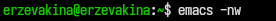
\includegraphics[width=0.7\linewidth,height=\textheight,keepaspectratio]{image/л11з1.png}
\caption{Задание 1}\label{fig-001}
\end{figure}

\begin{enumerate}
\def\labelenumi{\arabic{enumi}.}
\setcounter{enumi}{1}
\item
  Создать файл lab07.sh с помощью комбинации Ctrl-x Ctrl-f (C-x C-f).
\item
  Наберите текст:
\end{enumerate}

\begin{verbatim}
#!/bin/bash
HELL=Hello
function hello {
LOCAL HELLO=World
echo $HELLO
}
echo $HELLO
hello
\end{verbatim}

{[}рис. @fig-002{]}

\begin{figure}
\centering
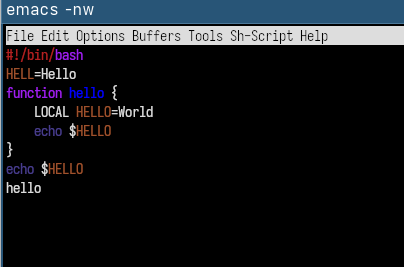
\includegraphics[width=0.7\linewidth,height=\textheight,keepaspectratio]{image/л11з3.png}
\caption{Задание 3}\label{fig-002}
\end{figure}

\begin{enumerate}
\def\labelenumi{\arabic{enumi}.}
\setcounter{enumi}{3}
\tightlist
\item
  Сохранить файл с помощью комбинации Ctrl-x Ctrl-s (C-x C-s).
\end{enumerate}

{[}рис. @fig-003{]}

\begin{figure}
\centering
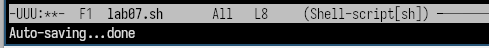
\includegraphics[width=0.7\linewidth,height=\textheight,keepaspectratio]{image/л11з4.png}
\caption{Задание 4}\label{fig-003}
\end{figure}

\begin{enumerate}
\def\labelenumi{\arabic{enumi}.}
\setcounter{enumi}{4}
\tightlist
\item
  Проделать с текстом стандартные процедуры редактирования, каждое
  действие должно осуществляться комбинацией клавиш.
\end{enumerate}

\begin{itemize}
\item
  Вырезать одной командой целую строку (С-k). {[}рис. @fig-004{]}
  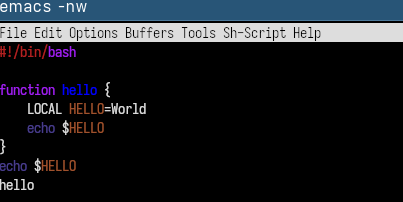
\includegraphics[width=0.7\linewidth,height=\textheight,keepaspectratio]{image/л11з5с1.png}
\item
  Вставить эту строку в конец файла (C-y). {[}рис. @fig-005{]}
  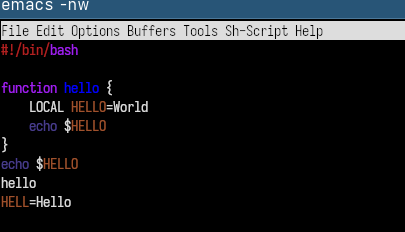
\includegraphics[width=0.7\linewidth,height=\textheight,keepaspectratio]{image/л11з5_с2.png}
\item
  Выделить область текста (C-space).
\item
  Скопировать область в буфер обмена (M-w). {[}рис. @fig-006{]}
  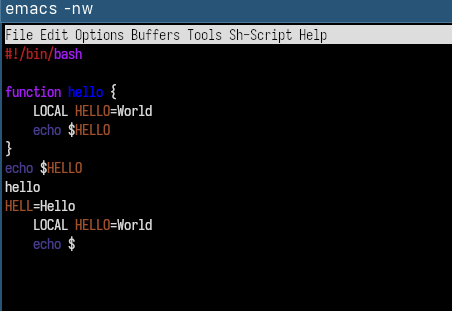
\includegraphics[width=0.7\linewidth,height=\textheight,keepaspectratio]{image/л11з5с4.png}
\item
  Вставить область в конец файла. {[}рис. @fig-007{]}
  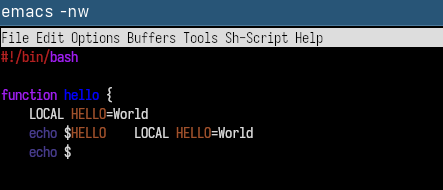
\includegraphics[width=0.7\linewidth,height=\textheight,keepaspectratio]{image/л11з5с5.png}
\item
  Вновь выделить эту область и на этот раз вырезать её (C-w).
\item
  Отмените последнее действие (C-/). {[}рис. @fig-008{]}
  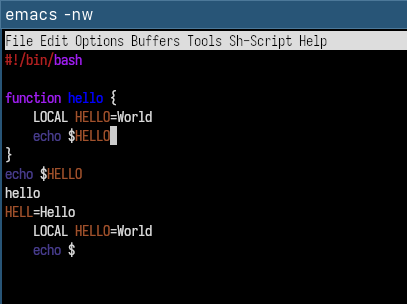
\includegraphics[width=0.7\linewidth,height=\textheight,keepaspectratio]{image/л11з5с7.png}
\end{itemize}

\begin{enumerate}
\def\labelenumi{\arabic{enumi}.}
\setcounter{enumi}{5}
\tightlist
\item
  Научитесь использовать команды по перемещению курсора.
\end{enumerate}

\begin{itemize}
\item
  Переместите курсор в начало строки (C-a). {[}рис. @fig-009{]}
  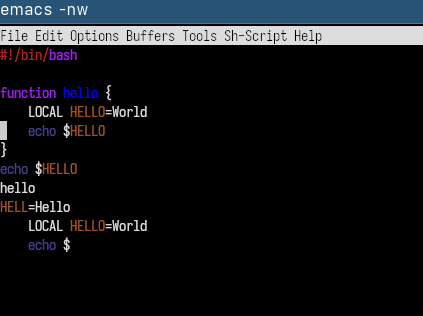
\includegraphics[width=0.7\linewidth,height=\textheight,keepaspectratio]{image/л11з6с1.png}
\item
  Переместите курсор в конец строки (C-e). {[}рис. @fig-010{]}
  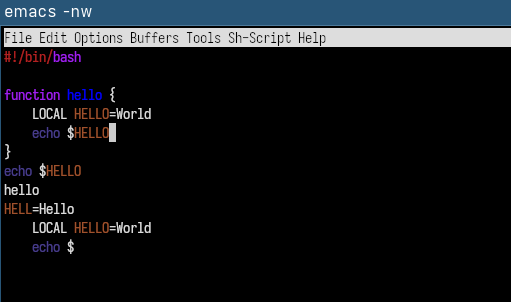
\includegraphics[width=0.7\linewidth,height=\textheight,keepaspectratio]{image/л11з6с2.png}
\item
  Переместите курсор в начало буфера (M-\textless).
\item
  Переместите курсор в конец буфера (M-\textgreater). {[}рис.
  @fig-011{]}
  
\includegraphics[width=0.7\linewidth,height=\textheight,keepaspectratio]{image/л11з6с4.png}
\end{itemize}

\begin{enumerate}
\def\labelenumi{\arabic{enumi}.}
\setcounter{enumi}{6}
\tightlist
\item
  Управление буферами.
\end{enumerate}

\begin{itemize}
\item
  Вывести список активных буферов на экран (C-x C-b). {[}рис.
  @fig-012{]}
  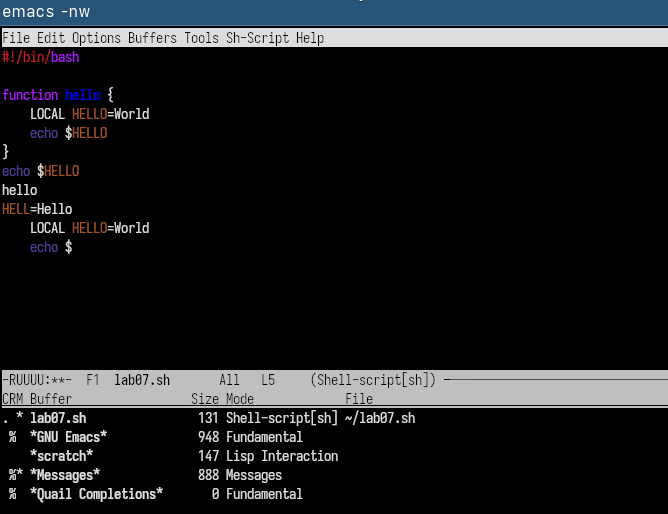
\includegraphics[width=0.7\linewidth,height=\textheight,keepaspectratio]{image/л11з7с1.png}
\item
  Переместитесь во вновь открытое окно (C-x) o со списком открытых
  буферов и переключитесь на другой буфер. {[}рис. @fig-013{]}
  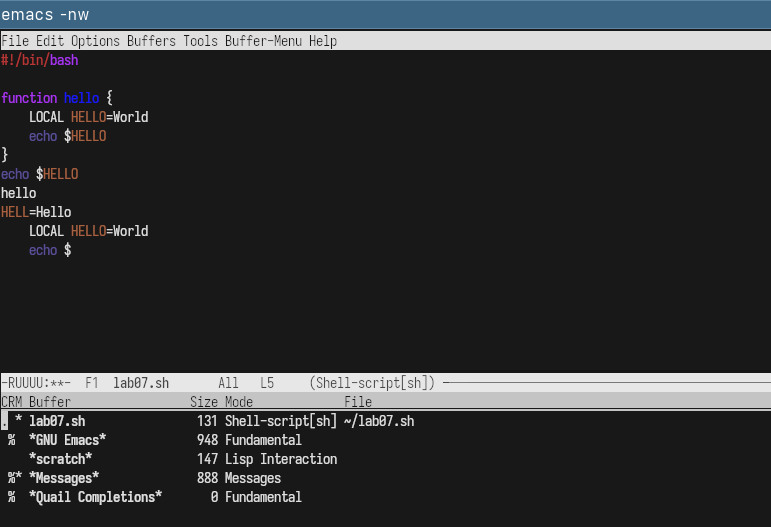
\includegraphics[width=0.7\linewidth,height=\textheight,keepaspectratio]{image/л11з7с2.png}
\item
  Закройте это окно (C-x 0). {[}рис. @fig-014{]}
  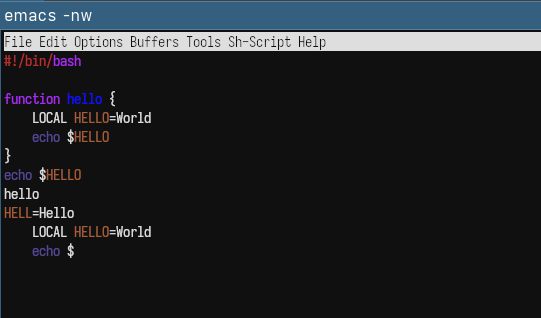
\includegraphics[width=0.7\linewidth,height=\textheight,keepaspectratio]{image/л11з7с3.png}
\item
  Теперь вновь переключайтесь между буферами, но уже без вывода их
  списка на экран (C-x b). {[}рис. @fig-015{]}
  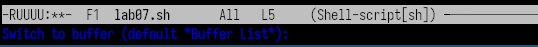
\includegraphics[width=0.7\linewidth,height=\textheight,keepaspectratio]{image/л11з7с4.png}
\end{itemize}

\begin{enumerate}
\def\labelenumi{\arabic{enumi}.}
\setcounter{enumi}{7}
\tightlist
\item
  Управление окнами.
\end{enumerate}

\begin{itemize}
\item
  Поделите фрейм на 4 части: разделите фрейм на два окна по вертикали
  (C-x 3), а затем каждое из этих окон на две части по горизонтали (C-x
  2) (см. рис. 9.1) {[}рис. @fig-016{]}
  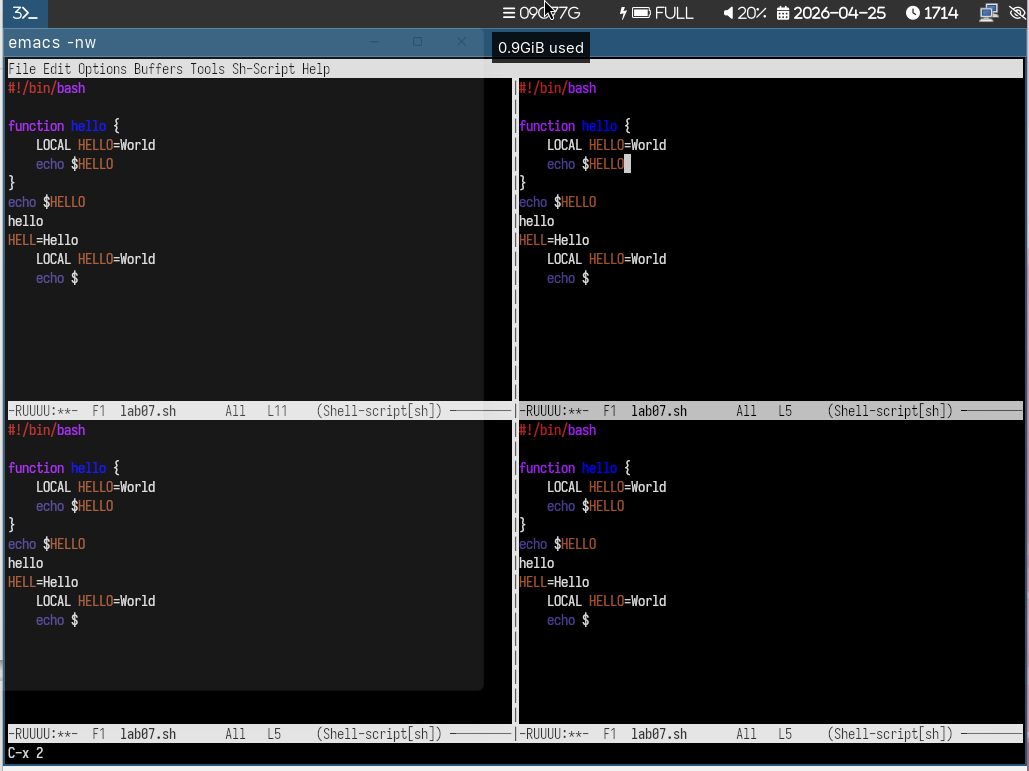
\includegraphics[width=0.7\linewidth,height=\textheight,keepaspectratio]{image/л11з8с1.png}
\item
  В каждом из четырёх созданных окон откройте новый буфер (файл) и
  введите несколько строк текста. {[}рис. @fig-017{]}
  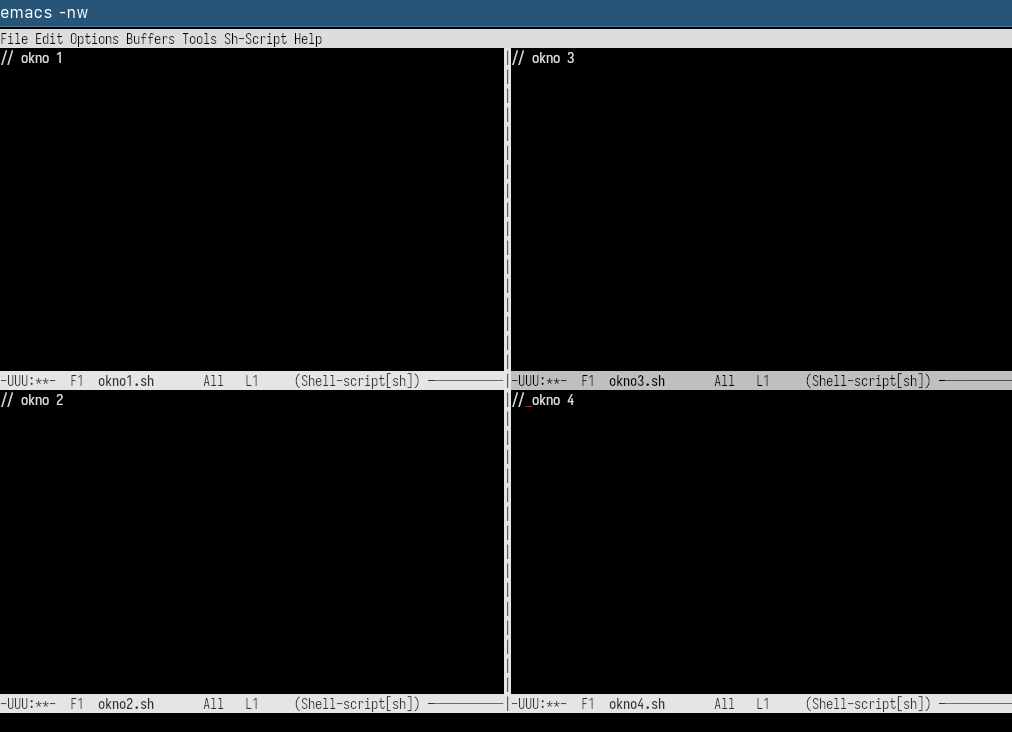
\includegraphics[width=0.7\linewidth,height=\textheight,keepaspectratio]{image/л11з8с2.png}
\end{itemize}

\begin{enumerate}
\def\labelenumi{\arabic{enumi}.}
\setcounter{enumi}{8}
\tightlist
\item
  Режим поиска
\end{enumerate}

\begin{itemize}
\item
  Переключитесь в режим поиска (C-s) и найдите несколько слов,
  присутствующих в тексте. {[}рис. @fig-018{]}
  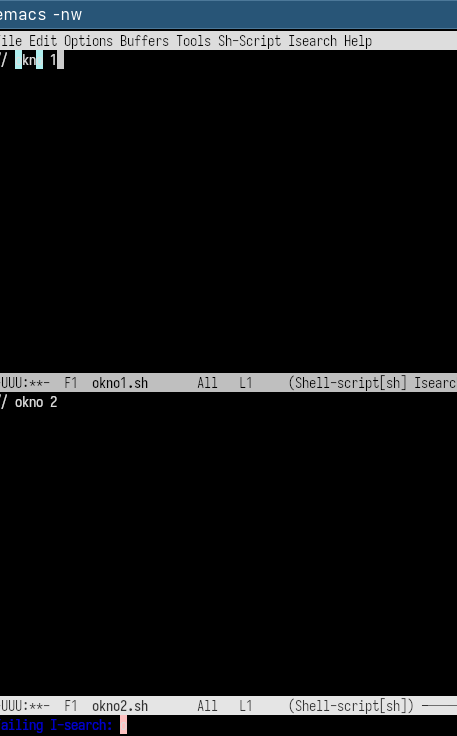
\includegraphics[width=0.7\linewidth,height=\textheight,keepaspectratio]{image/л11з9с1.png}
\item
  Переключайтесь между результатами поиска, нажимая C-s. {[}рис.
  @fig-019{]}
  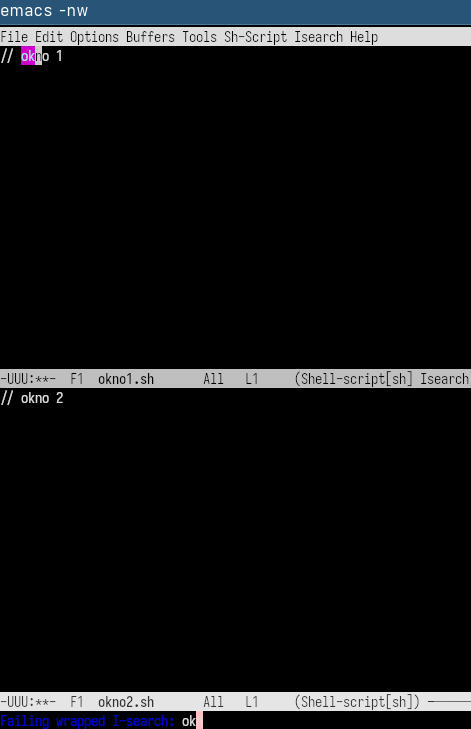
\includegraphics[width=0.7\linewidth,height=\textheight,keepaspectratio]{image/л11з9с2.png}
\item
  Выйдите из режима поиска, нажав C-g. {[}рис. @fig-020{]}
  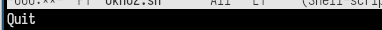
\includegraphics[width=0.7\linewidth,height=\textheight,keepaspectratio]{image/л11з9с3.png}
\item
  Перейдите в режим поиска и замены (M-\%), введите текст, который
  следует найти и заменить, нажмите Enter , затем введите текст для
  замены. После того как будут подсвечены результаты поиска, нажмите !
  для подтверждения замены. {[}рис. @fig-021{]}
  
\includegraphics[width=0.7\linewidth,height=\textheight,keepaspectratio]{image/л11з9с4.png}
\item
  Испробуйте другой режим поиска, нажав M-s o. Объясните, чем он
  отличается от обычного режима? {[}рис. @fig-022{]}
  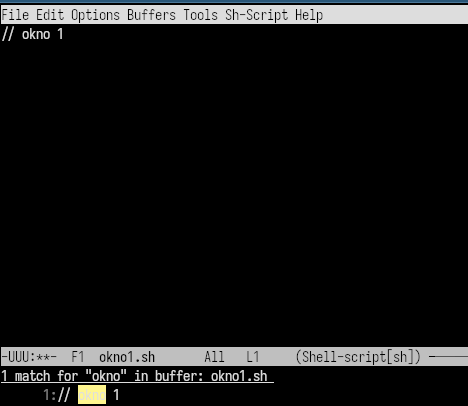
\includegraphics[width=0.7\linewidth,height=\textheight,keepaspectratio]{image/л11з9с5.png}
\end{itemize}

\chapter{Контрольные
вопросы}\label{ux43aux43eux43dux442ux440ux43eux43bux44cux43dux44bux435-ux432ux43eux43fux440ux43eux441ux44b}

\section{1. Кратко охарактеризуйте редактор
emacs.}\label{ux43aux440ux430ux442ux43aux43e-ux43eux445ux430ux440ux430ux43aux442ux435ux440ux438ux437ux443ux439ux442ux435-ux440ux435ux434ux430ux43aux442ux43eux440-emacs.}

Ответ: Emacs --- это мощный расширяемый текстовый редактор, который
используется для программирования, работы с текстами, управления
файлами, почтой, терминалом и многими другими задачами. Его часто
называют не просто редактором, а целой рабочей средой.

\section{2. Какие особенности данного редактора могут сделать его
сложным для освоения
новичком?}\label{ux43aux430ux43aux438ux435-ux43eux441ux43eux431ux435ux43dux43dux43eux441ux442ux438-ux434ux430ux43dux43dux43eux433ux43e-ux440ux435ux434ux430ux43aux442ux43eux440ux430-ux43cux43eux433ux443ux442-ux441ux434ux435ux43bux430ux442ux44c-ux435ux433ux43e-ux441ux43bux43eux436ux43dux44bux43c-ux434ux43bux44f-ux43eux441ux432ux43eux435ux43dux438ux44f-ux43dux43eux432ux438ux447ux43aux43eux43c}

Ответ: Новичкам Emacs может показаться сложным из-за: - большого
количества сочетаний клавиш; - необычной системы команд (например, C-x
C-f); - большого числа встроенных режимов и настроек; - непривычной
терминологии (буферы, окна, фреймы); - необходимости запоминать команды
вместо работы только через меню.

\section{3. Своими словами опишите, что такое буфер и окно в
терминологии
emacs'а.}\label{ux441ux432ux43eux438ux43cux438-ux441ux43bux43eux432ux430ux43cux438-ux43eux43fux438ux448ux438ux442ux435-ux447ux442ux43e-ux442ux430ux43aux43eux435-ux431ux443ux444ux435ux440-ux438-ux43eux43aux43dux43e-ux432-ux442ux435ux440ux43cux438ux43dux43eux43bux43eux433ux438ux438-emacsux430.}

Ответ: \textbf{Буфер} --- это содержимое открытого файла (или служебная
область), с которым работает Emacs в памяти. \textbf{Окно} --- это
область экрана, в которой отображается буфер. Одно окно показывает один
буфер, но один и тот же буфер можно показывать в разных окнах.

\section{4. Можно ли открыть больше 10 буферов в одном
окне?}\label{ux43cux43eux436ux43dux43e-ux43bux438-ux43eux442ux43aux440ux44bux442ux44c-ux431ux43eux43bux44cux448ux435-10-ux431ux443ux444ux435ux440ux43eux432-ux432-ux43eux434ux43dux43eux43c-ux43eux43aux43dux435}

Ответ: Да, можно. Количество буферов практически не ограничено, и их
может быть намного больше 10. В одном окне одновременно отображается
только один буфер, но переключаться можно между любым количеством
буферов.

\section{5. Какие буферы создаются по умолчанию при запуске
emacs?}\label{ux43aux430ux43aux438ux435-ux431ux443ux444ux435ux440ux44b-ux441ux43eux437ux434ux430ux44eux442ux441ux44f-ux43fux43e-ux443ux43cux43eux43bux447ux430ux43dux438ux44e-ux43fux440ux438-ux437ux430ux43fux443ux441ux43aux435-emacs}

Ответ: Обычно при запуске создаются: - буфер \emph{scratch} --- для
временных заметок и Lisp-кода; - буфер \emph{Messages} --- для служебных
сообщений редактора.

\section{6. Какие клавиши вы нажмёте, чтобы ввести следующую комбинацию
C-c \textbar{} и C-c
C-\textbar?}\label{ux43aux430ux43aux438ux435-ux43aux43bux430ux432ux438ux448ux438-ux432ux44b-ux43dux430ux436ux43cux451ux442ux435-ux447ux442ux43eux431ux44b-ux432ux432ux435ux441ux442ux438-ux441ux43bux435ux434ux443ux44eux449ux443ux44e-ux43aux43eux43cux431ux438ux43dux430ux446ux438ux44e-c-c-ux438-c-c-c-}

Ответ: - C-c \textbar{} → удерживать Ctrl, нажать c, отпустить, затем
нажать Shift + ~(символ \textbar) - C-c C-\textbar{} → удерживать Ctrl,
нажать c, затем, не отпуская Ctrl, нажать Ctrl + Shift +\\

\section{7. Как поделить текущее окно на две
части?}\label{ux43aux430ux43a-ux43fux43eux434ux435ux43bux438ux442ux44c-ux442ux435ux43aux443ux449ux435ux435-ux43eux43aux43dux43e-ux43dux430-ux434ux432ux435-ux447ux430ux441ux442ux438}

Ответ: Поделить текущее окно на две части можно командой: - C-x 2 ---
горизонтальное разделение (одно над другим) - C-x 3 --- вертикальное
разделение (рядом друг с другом)

\section{8. В каком файле хранятся настройки редактора
emacs?}\label{ux432-ux43aux430ux43aux43eux43c-ux444ux430ux439ux43bux435-ux445ux440ux430ux43dux44fux442ux441ux44f-ux43dux430ux441ux442ux440ux43eux439ux43aux438-ux440ux435ux434ux430ux43aux442ux43eux440ux430-emacs}

Ответ: Настройки Emacs обычно хранятся в файле: - \textasciitilde/.emacs
или - \textasciitilde/.emacs.d/init.el

\section{9. Какую функцию выполняет клавиша и можно ли её
переназначить?}\label{ux43aux430ux43aux443ux44e-ux444ux443ux43dux43aux446ux438ux44e-ux432ux44bux43fux43eux43bux43dux44fux435ux442-ux43aux43bux430ux432ux438ux448ux430-ux438-ux43cux43eux436ux43dux43e-ux43bux438-ux435ux451-ux43fux435ux440ux435ux43dux430ux437ux43dux430ux447ux438ux442ux44c}

Ответ: Клавиша стрелка влево перемещает курсор на один символ влево
(аналог команды backward-char).

Да, её можно переназначить, так как в Emacs почти любую клавишу можно
изменить через настройку key bindings.

\section{10. Какой редактор вам показался удобнее в работе vi или emacs?
Поясните
почему.}\label{ux43aux430ux43aux43eux439-ux440ux435ux434ux430ux43aux442ux43eux440-ux432ux430ux43c-ux43fux43eux43aux430ux437ux430ux43bux441ux44f-ux443ux434ux43eux431ux43dux435ux435-ux432-ux440ux430ux431ux43eux442ux435-vi-ux438ux43bux438-emacs-ux43fux43eux44fux441ux43dux438ux442ux435-ux43fux43eux447ux435ux43cux443.}

Ответ: Мне удобнее Emacs, потому что он более гибкий и расширяемый:
можно настроить почти всё под себя, использовать встроенные инструменты
и писать собственные команды. Однако vi удобнее для быстрых правок в
терминале, так как он легче и быстрее запускается. Для постоянной работы
я бы выбрал Emacs, а для срочного редактирования --- vi.

\chapter{Выводы}\label{ux432ux44bux432ux43eux434ux44b}

\chapter*{Список
литературы}\label{ux441ux43fux438ux441ux43eux43a-ux43bux438ux442ux435ux440ux430ux442ux443ux440ux44b}
\addcontentsline{toc}{chapter}{Список литературы}

\protect\phantomsection\label{refs}

\printbibliography

\end{document}
